
%%%%%%%%%%%%%%%%%%%%%%%%%%%%%%%%%%%%%%%%%%%%%%%%%%%%%%%%%%%%%%%%%%% 
%                                                                 %
%                           METHODS                               %
%                                                                 %
%%%%%%%%%%%%%%%%%%%%%%%%%%%%%%%%%%%%%%%%%%%%%%%%%%%%%%%%%%%%%%%%%%% 
 
% \specialhead{METHODS}
\chapter{VISUALIZATION}
\label{chapter:visualization}
As stated in Chapter~\ref{chapter:intro}, this thesis work started as a proof of concept for performing
real-time fisheye deformations on Graphics Processing Units(GPU) using OpenGL 3.1. The previous version of the visualization application used the OpenGL 2.0 specifications (referred to as legacy OpenGL from here on). OpenGL 3.0 specifications were released in September 2008, labeling many of the core functions as deprecated \cite{opengl_3_specification}. In Sections~\ref{section:legacy_opengl} and~\ref{section:modern_opengl}, a brief description of the relevant deprecated
functionality and the replacement methods is given. Section~\ref{section:base_mapview_elements} discusses the implementation details for upgrading the core functionality of the graph visualization. Finally, Section~\ref{section:satellite_images} and Section~\ref{section:road_network} details the rendering process of the satellite images and road network.

\section{Legacy OpenGL}
\label{section:legacy_opengl}

The standard for rendering polygons in legacy OpenGL was immediate mode. The functions {\tt glBegin()} 
and {\tt glEnd()} indicate that the calls to {\tt glVertex()} form a polygon specified by the call to {\tt glBegin().} 
All vertices specified this way can also have texture coordinates, colors, and normal vectors 
passed to OpenGL for rendering. These shapes are drawn immediately to the buffer after the 
call to {\tt glEnd().} Listing~\ref{lst:simple_triangle} shows a code sample for rendering a colored triangle in legacy OpenGL. 

\begin{lstlisting}[float, 
    caption={[Legacy OpenGL Colored Triangle] Rendering a triangle with a red, blue, and green corner.},
    label={lst:simple_triangle}]
glBegin(GL_TRIANGLES);
glColor3f( 1.0, 0.0, 0.0);
glVertex2f( 0.0, 1.0 );
glColor3f( 0.0, 1.0, 0.0):
glVertex2f( 1.0, -1.0 );
glColor3f( 0.0, 0.0, 1.0);
glVertex2f( -1.0, -1.0 );
glEnd()
\end{lstlisting}

Rendering in a 3D environment involves the transformation of vertex positions. First the coordinates 
are transformed from object space to world space, where object space has vertices defined relative 
to an object's center point and world space has vertices defined relative to all other objects 
within the world. Defining objects in world space places objects within the world, akin to placing props on a stage. The coordinates are then transformed to eye space, which represents their 
positions relative to the viewer. The viewer is assumed to be at the origin in world space, looking in the negative z direction. Eye space is useful for defining how far away any particular object is from the viewer, which is represented as the z direction.  Finally, eye space is transformed  to projection space, where objects are projected onto a 2D screen based on their positions and distance from the user. Each of the respective transformations are represented by different matrices. The model, view, and projection matrices correspond to the transformation to world, eye, and projection space, respectively \cite{opengl_matrix_stack}. 

In legacy OpenGL, these matrices were handled by a matrix stack ({\tt glPopMa\-trix(),} {\tt glPushMatrix()).} 
The model and view matrices were combined into a single matrix for OpenGL, represented by the 
constant {\tt GL\_MODELVIEW\@}. The projection matrix, {\tt GL\_PROJECTION}, was handled by either {\tt glOrtho()} 
or {\tt glFrustum()} for either an orthographic or standard projection.

Because we are rendering a 2D environment, we use an orthographic projection to ensure that 
objects are not scaled by the environment based on their distance away from the camera, this ensures that changing the level of detail of the overall system does not cause objects to become too small to perceive or to become too large to view anything else. An orthographic projection allows us to utilize the z dimension as a method of choosing the order in which elements should be displayed, i.e.\ which elements will be drawn over other elements within the overall application.

\section{Modern OpenGL}
\label{section:modern_opengl}

Our application uses OpenGL 3.2 specifically to use geometry shaders as part of our core functionality. Version 3.0 of OpenGL marked functions in legacy OpenGL as deprecated, but they were not officially removed from the core profile until OpenGL 3.1. To avoid further confusion between different versions, we will refer to OpenGL 3.2 as modern OpenGL.

Passing vertex data to OpenGL via the above method of {\tt glBegin()} and {\tt glEnd()} was deprecated for modern OpenGL\@. Rendering now requires the usage of vertex and fragment shaders, 
programs that run on the Graphics Processing Unit (GPU) and operate on vertices and the interpolated 
screen fragments surrounded by the vertices.  The previous methods for changing attributes of a particular vertex relied on the fixed function pipeline. This change was introduced due to the overall flexibility of shaders. While shaders are more expressive than the fixed function pipeline of legacy OpenGL, they require more code for simple tasks.

In a standard draw function using modern OpenGL, data is specified in Vertex Buffer Objects (VBOs) 
which contains the data that is sent to the vertex shader. VBOs are the GPU equivalent of Vertex Arrays, batches of vertex data stored in CPU address space. Vertex Arrays were deprecated as their performance when compared with VBOs were much worse due to requiring data to be transfer ed to the GPU on every frame. VBOs provide a mechanism for utilizing GPU memory within OpenGL~\cite{opengl_3_specification}. VBOs contain the same data that 
would be called between the {\tt glBegin()} and {\tt glEnd()} calls, and are created and activated with 
the {\tt glGenBuffers()} and {\tt glBindBuffer()} commands. The function {\tt glBufferData()} allocates memory for the data on the GPU and is given a pointer to sequential memory that will be copied into the GPU\@. Different VBOs or regions of memory are then referred to by vertex attribute pointers using the {\tt glVertexAttribPointer()} function. These pointers inform the vertex shaders how to interpret the data. If necessary, any extra data can be passed to the vertex and fragment shaders via calls to {\tt glUniform()}. The two commands, {\tt glDrawArrays()} and {\tt glDrawElements()}, are used to specify a range of data to be drawn by OpenGL, sending data as necessary.

Listing~\ref{lst:modern_triangle} shows a C++ code sample of specifying the same triangle in Listing~\ref{lst:simple_triangle} with modern OpenGL\@. Listing~\ref{lst:vertex_shader} and~\ref{lst:fragment_shader} show the necessary vertex and fragment shaders, respectively.

%\lstinputlisting[ caption={[Modern OpenGL C++ Colored Triangle]Rendering a triangle with a red, blue, and green 
%    corner. The C++ code generates the necessary VBO, one for position and one for color, inserts the data, and 
%    then renders the triangle.},
%    label={lst:modern_triangle}]
%{data/modern_triangle.cpp}

%\lstinputlisting[ caption={[Colored Triangle Vertex Shader]The vertex shader for {\tt triangleProgram}. The 
%    shader receives the position and color data and passes this information to the fragment shader through the 
%    out variable.},
%    label={lst:vertex_shader}]
%{data/simple.vert}

%\lstinputlisting[ caption={[Colored Triangle Fragment Shader]The fragment shader for {\tt triangleProgram}. The 
%    shader receives the interpolated color and position from the vertex shader and outputs data to the screen.},   
%    label={lst:fragment_shader}]
%{data/simple.frag}

Functionality related to the matrix stack was also deprecated for modern OpenGL\@. Developers must now manage their own matrices and vectors. This was another side effect of removing the fixed function pipeline. Much like the addition of shaders, the modern OpenGL specification made this change to allow for greater flexibility. Developers do not have to conform to using the {\tt GL\_MODELVIEW} and {\tt GL\_PROJECTION} matrices for their transformations. The GLM library
\cite{glm_website} was developed to duplicate this missing functionality and act as a CPU implementation of the OpenGL Shader Language (GLSL) vector and matrix operations. These matrices and other variables are passed to the shaders as uniform variables (variables that are constant across all invocations of a shader). The vertex shader is now responsible for performing any relevant operations on a per-vertex basis. These operations include transforming a vertex's position in model or
world space to projection space and light calculations based on a vertex's normal vector. After this step, coordinates are expected to be in Normalized Device Coordinates (NDC), which range from -1 to 1 in the x, y, and z directions. The area between a triangle is then broken into different fragments. Any data that was stored in the three vertices is interpolated over this entire region. Each of these fragments is operated on by the fragment shader. The fragment shader is
responsible for choosing the resulting color of a particular fragment before the scene is rendered to the display.

While vertex and fragment shaders are mandatory due to their equivalent functionality being removed from the fixed function pipeline, geometry shaders provide an optional method of manipulating vertex data on the GPU\@. Given input data in the form of points, lines, or triangles, the geometry shader is able to modify vertex data between the vertex and fragment shaders. Figure~\ref{fig:shader_pipeline} shows the OpenGL shader pipeline for the infrastructure visualization.

\begin{figure}[htp] \centering
    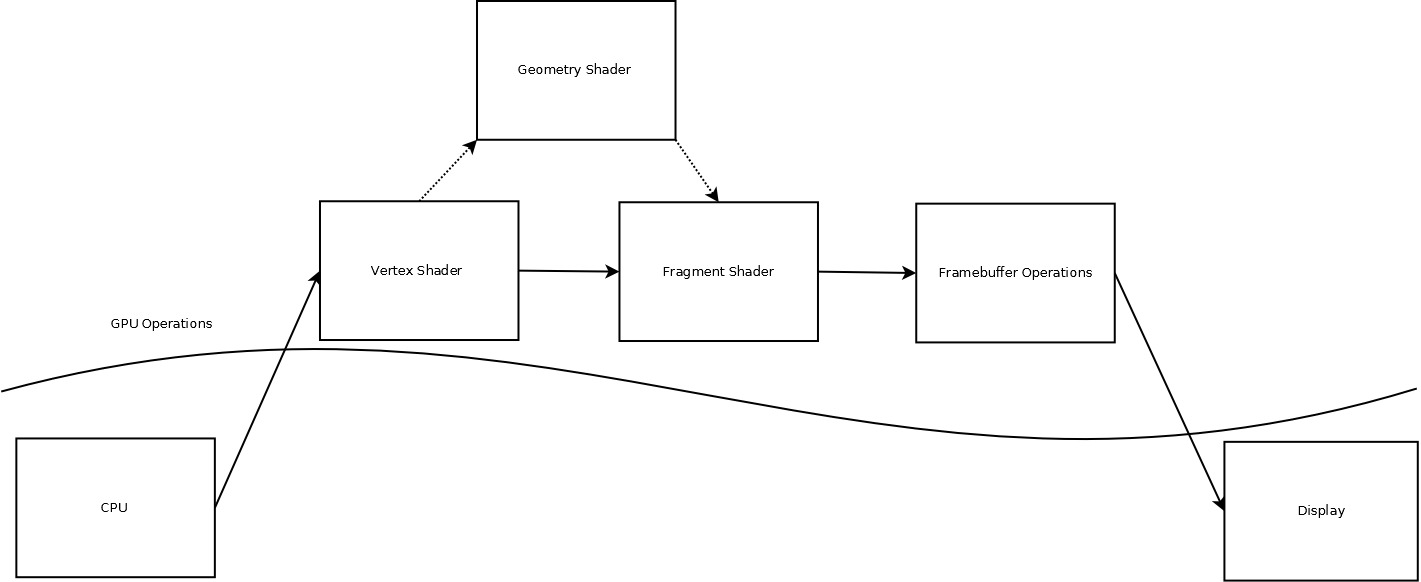
\includegraphics[width=150mm]{img/pipeline.jpg}
    \caption[Infrastructure Visualization Shader Pipeline]{An overview of the visualization's shader pipeline.}
    \label{fig:shader_pipeline}
\end{figure}

\section{Base Visualization Elements}
\label{section:base_mapview_elements}

The following sections, describe the rendering methods of different base elements that are used in different places throughout the entire application. Each section explains the usage of individual elements, describes the method used in the previous versions of the visualization for rendering, and is concluded by the method used for modern OpenGL compliance.

\subsection{Buttons}
\label{subsection:buttons}
For the visualization, buttons are the nodes of the graph network. Their default state is a circle such that all nodes of a particular resource are colored the same. When expanded, these elements increase in area and take on the shape of squares. These squares are then overlaid by text describing relevant status information. This visual change is to allow users to easily pick out nodes which have more information, as well as to allow for more space for text to be drawn. Every button has at least one associated border
with it in an attempt to provide further distinction between nearby nodes. Multiple borders surrounding a node indicates that a node is not receiving the resource associated with the color. Figure~\ref{fig:buttons} shows two nodes, one expanded and the other unexpanded.

\begin{figure}[htp] \centering
    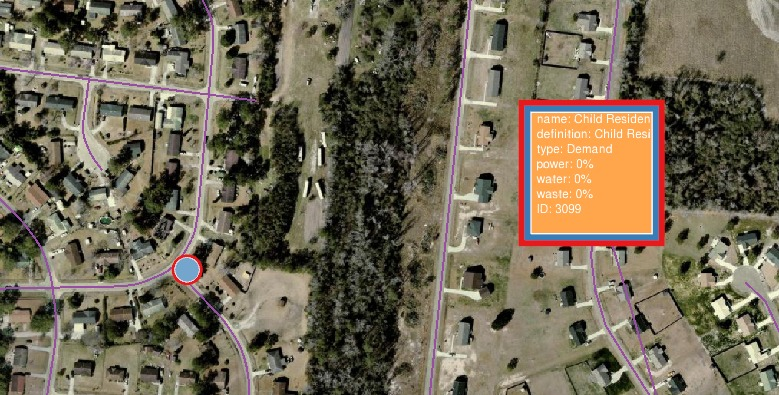
\includegraphics[width=0.8\linewidth]{img/buttons.jpg}
    \caption[Buttons]{An image showing two nodes of the graph network. The expanded node has a significantly greater area than the unexpanded node. Both nodes have a red border, indicating a lack of power. The expanded node has a lack of water as well, shown by the blue border.}
    \label{fig:buttons}
\end{figure}

The implementation of drawing buttons in the legacy OpenGL code followed the format of the 
pseudocode seen in Algorithm~\ref{alg:button_drawing}.

\begin{algorithm}
    \caption{Pseudocode detailing the general process of rendering a button in the legacy OpenGL
    version of the visualization.}\label{alg:button_drawing}
    \begin{algorithmic}[1]
        \Function{Button Drawing}{}
            \ForAll{Button in Buttons}
                \If{Button is not expanded}
                \State\Call{DrawCircleBorder}{Button}
                    \If{Button is textured}
                        \State\Call{DrawCircleTexturedButton}{Button}
                    \Else
                        \State\Call{DrawCircleUntexturedButton}{Button}
                    \EndIf
                \Else
                    \State\Call{DrawRectangleBorder}{Button}
                    \If{Button is textured}
                        \State\Call{DrawRectangleTexturedButton}{Button}
                    \Else
                        \State\Call{DrawRectangleUntexturedButton}{Button}
                    \EndIf
                    \If{Button has text}
                        \State\Call{DrawText}{Button}
                    \EndIf
                \EndIf
            \EndFor
        \EndFunction
    \end{algorithmic}
\end{algorithm}

The borders representing state data are drawn first, followed by either an untextured or textured 
main button area. Finally, if a button is expanded and has corresponding text, the text is 
also drawn. A button and all of its related elements (text and borders) are given the same z value when rendered. This z value is the ``depth'' of the element within the overall scene relative to the camera, such that elements with a lower z value are closer to the camera, and elements with a higher z value are further away. Because we are using an orthographic projection, this information allows us to choose the order in which we render objects.OpenGL provides methods for determining if a
new pixel should be drawn based on the information in the depth buffer. A call to {\tt glDepthFunc(GL\_LEQUAL)} tells OpenGL that the current pixel in a location should be discarded if the new pixel has a z value less than or equal to the current amount stored in the depth buffer \cite{opengl_depth_buffer}. This method of The drawing order is important to note, as elements with the same z order will be drawn in the order that calls to {\tt glDrawArrays()} are performed, this is known
as the Painter's algorithm \cite{Berg1993}. In the previous version of OpenGL, the entirety of the layering was handled by Painter's algorithm, requiring all of the buttons in the application to be sorted every frame. Figure~\ref{fig:layering_buttons} shows the layering of buttons.

\begin{figure}[htp] \centering
    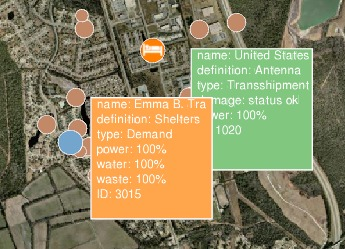
\includegraphics[width=0.8\linewidth]{img/button_layering.jpg}
    \caption[Button Layering]{Elements that have been interacted with have a lower z value and are drawn over other buttons. Text has the same z value as the underlying button, but is drawn later, so is still visible on the expanded.}
    \label{fig:layering_buttons}
\end{figure}

The drawing of buttons and their borders relied on two drawing formats in legacy OpenGL that were 
completely removed in OpenGL 3.1, {\tt GL\_QUADS} and {\tt GL\_POLYGON\@}. Duplicating the {\tt GL\_QUADS} functionality 
is trivial with {\tt GL\_TRIANGLES} or {\tt GL\_TRIANGLE\_STRIP\@}. For a quadrilateral with vertices a, b, 
c, d, create one triangle with vertices a, b, c and one with vertices a, c, d. We elected to 
use {\tt GL\_TRIANGLES}, as {\tt GL\_TRIANGLE\_STRIP} indicates that the entire range of vertices passed to
{\tt glDrawArrays()} is a continuous strip of triangles, and would necessitate multiple function 
calls to draw multiple rectangular buttons.

{\tt GL\_POLYGON} allowed a user to specify a convex polygon with $N$ sides. This was used to create 
a 20-sided polygon to approximate the appearance of a circle. Every adjacent pair of vertices 
specified forms one edge, with vertices 1 and $N$ forming the last edge of the polygon. There are a few choices for replicating {\tt GL\_POLYGON} functionality. {\tt GL\_TRIANGLE\_FAN} best approximates 
the old functionality by taking a center vertex and forming individual triangles out of every 
adjacent pair of vertices and the center vertex. Using {\tt GL\_TRIANGLE\_FAN} reduces the number of vertices that have to be specified to draw a circle. Unfortunately, this approach has the same 
downside that using {\tt GL\_TRIANGLE\_STRIP} for drawing rectangular buttons has, drawing $N$ circles 
with this method requires $N$ calls to {\tt glDrawArrays()}, as all vertices in the range passed to {\tt glDrawArrays()} are considered to be connected to the first vertex specified. Much like drawing rectangular buttons, using {\tt GL\_TRIANGLES}
allows for all of the circular buttons to be drawn in one call to {\tt glDrawArrays().}

Replacing the old functionality was considered, but the individual buttons never stored the 
vertex data for {\tt GL\_POLYGON}, it was simply computed as needed based on a center point, and a 
radius. Instead of calculating these new triangles on every frame on the CPU, we chose to use a geometry 
shader, which performs the same operations but specifies 59 less vertices and can be computed in parallel. To generate a circular button, the geometry shader constructs 20 triangles with the 
following algorithm (Algorithm~\ref{alg:circle_geometry}). 

\begin{algorithm}
    \caption{Creating a circle from 20 individual triangles given a center point and a radius. This can be implemented on the CPU or the GPU.}
    \label{alg:circle_geometry}
    \begin{algorithmic}[1]
        \Function{CreateCircle}{$\vec{center}$, $radius$}
        \For{$i=0 \rightarrow 20$}
            \State $a_0 = \frac{2\pi(i \% 20 )}{20}$ 
            \State $a_1 = \frac{2\pi((i+1) \% 20 )}{20}$ 

            \State $\vec{p_0} = \vec{center} + radius \times \langle cos(a_0), sin(a_0) \rangle$
            \State \Call{createVertex}{$\vec{p_0}$}

            \State \Call{createVertex}{$\vec{center}$}

            \State $\vec{p_1} = \vec{center} + radius \times \langle cos(a_1), sin(a_1) \rangle$
            \State \Call{createVertex}{$\vec{p_1}$}
        \EndFor
        \EndFunction
    \end{algorithmic}
\end{algorithm}

This algorithm replicates the functionality performed in the previous version of the visualization by 
generating triangles that have the center vertex and two vertices that are created by taking 
20 uniform samples of the circle expressed by the center vertex and the radius.

We use a total of four VBOs when rendering the buttons: Untextured circular buttons and circular borders,
Textured circular buttons, untextured rectangular buttons and rectangle borders, and textured rectangle 
buttons. The different types of buttons except the textured rectangle, as it is not currently used within the system, can be seen below.

The data in the VBOs change depending on the status of the button. If the underlying data representation changes, then the text of a button and its borders may change. When a button expands or contracts, data must be placed in different VBOs.

\begin{figure}[htp] \centering
    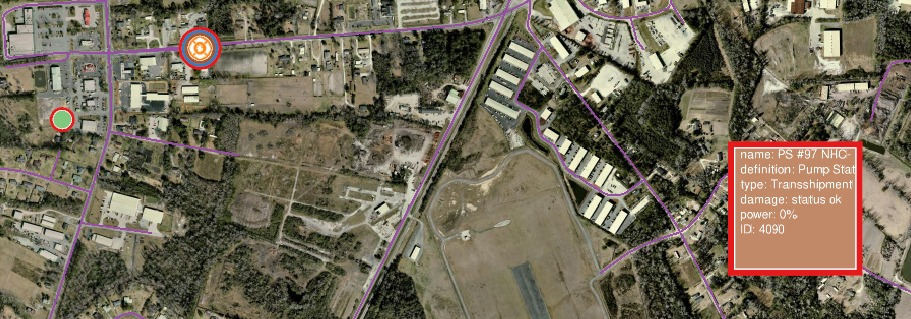
\includegraphics[width=0.8\linewidth]{img/button_types.jpg}
    \caption[Button Types]{An image showing the three types of buttons used within the visualization. From left to right, we see a untextured circular button, a textured circular button, and a untextured rectangle. The nodes are surrounded by colored borders that indicate problems with the supplied services. The button on the lower right is lacking power, hence the red border. The main button color indicates the service type, in this case brown represents the waste/sewage network. }
    \label{fig:button_types}
\end{figure}

\subsection{Lines}
\label{subsection:lines}

Drawing lines in modern OpenGL functions the same as drawing in legacy OpenGL with two major caveats. 
Legacy OpenGL allowed for calls to {\tt glLineWidth()} to set the integer width of drawn lines to a specific 
screen space value. This feature has been deprecated in OpenGL 3.1, resulting in the inability to 
have lines with a width greater than 1.0. Lines must also be passed into VBOs and rendered by a vertex and fragment shader.

To solve the line width problem, we utilize a geometry shader to create two triangles that form a quadrilateral 
that has a pixel width based on an input value. Pseudocode for the geometry shader is shown 
in Algorithm~\ref{alg:line_geometry}. In essence, the two endpoints of a line segment are pushed apart by half 
of the total width of the resulting line, generating four points total.

\begin{algorithm}
    \caption{Creating a rectangle from two triangles given the end points of a line segment and a width.}
    \label{alg:line_geometry}
    \begin{algorithmic}[1]
        \Function{CreateRectangle}{$\vec{p_0}$, $\vec{p_1}$, $width$}
        \State $dx = p_{1x} - p_{0x}$
        \State $dy = p_{1y} - p_{0y}$

        \State $\vec{normal} = \langle -dy \times \frac{width}{2}, dx \times \frac{width}{2}\rangle$
        \State $\vec{p_{00}} = \vec{p_0} + normal$
        \State $\vec{p_{01}} = \vec{p_0} - normal$

        \State $\vec{p_{10}} = \vec{p_1} + normal$
        \State $\vec{p_{11}} = \vec{p_1} - normal$

        \State \Call{createVertex}{$\vec{p_{00}}$}
        \State \Call{createVertex}{$\vec{p_{01}}$}
        \State \Call{createVertex}{$\vec{p_{10}}$}
        \State \Call{createVertex}{$\vec{p_{11}}$}

        \EndFunction
    \end{algorithmic}
\end{algorithm}

Drawing continuous lines with this method results in seeing disjoint areas where lines connect. 
To solve this graphical issue, we draw a circle at each endpoint with a radius equal to the width of the expanded line on the GPU using Algorithm~\ref{alg:circle_geometry}. Figure~\ref{fig:line_no_joint} shows a line segment without the circles drawn on the endpoints, and Figure~\ref{fig:line_joint} shows the same line segment with circular endpoints 

\begin{figure}[htp]
    \centering
    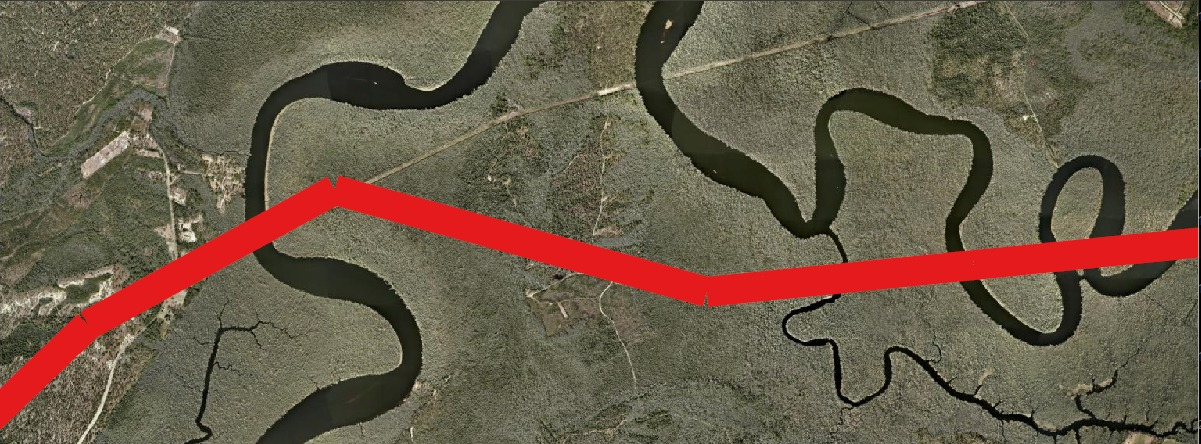
\includegraphics[width=0.90\linewidth]{img/expanded_edge_no_joint.jpg}
    \caption[Line Segment without Joints Drawn]{A line drawn by expanding multiple a line segments into rectangles. The individual segments are clearly visible due to the construction method.}
    \label{fig:line_no_joint}
\end{figure}
\begin{figure}[htp]
    \centering
    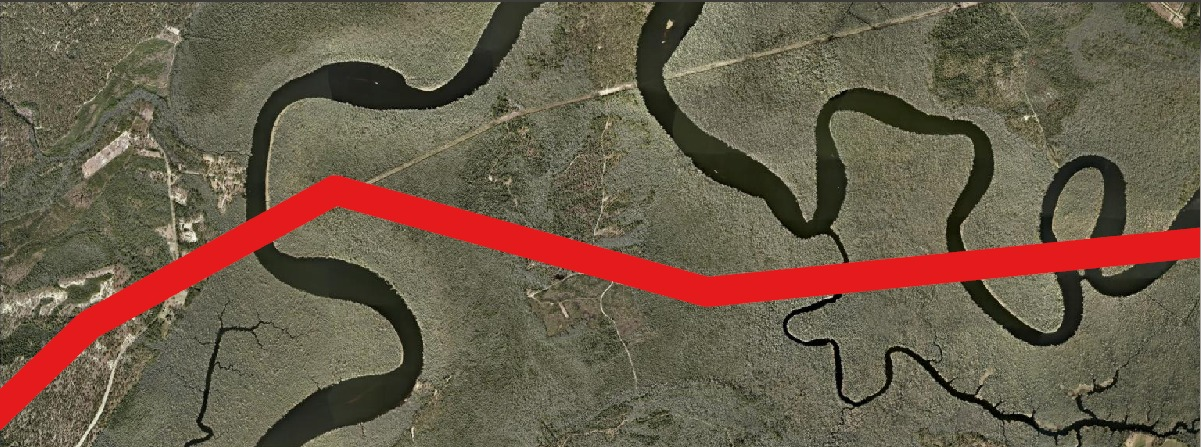
\includegraphics[width=0.90\linewidth]{img/expanded_edge_joint.jpg}
    \caption[Line Segments with Joints Drawn]{The same line as the Figure~\ref{fig:line_no_joint} but with circular joints drawn on the endpoints for the segments.}
    \label{fig:line_joint}
\end{figure}

The width of each line segment changes depending on if the overall graph edge in the network is expanded or not. These expanded lines have text drawn on them, displaying information about the status of transmitting a resource between the two nodes it connects. This status string is fairly short, and is therefore repeated over the entire length of the edge to ensure that the edge information is conveyed to the user. The figure below shows an example of an unexpanded line and an expanded line.

The previous version of the visualization used {\tt GL\_LINE\_STRIP} to draw individual line segments with only 
N vertices to represent a line with $N-1$ segments. Much like the issues discussed with rendering 
many buttons with {\tt GL\_TRIANGLE\_STRIP} in Section~\ref{subsection:buttons}, if individual lines continue to 
use the  {\tt GL\_LINE\_STRIP} format, $N$ calls to {\tt glDrawArrays()} are needed to draw $N$ different lines. While we do not have concrete timed data, the old method of rendering caused noticeable lag if the main source of lines, the road network, was being rendered. This lag would disappear if the road network was turned off. To sidestep 
this problem, we create individual line segments out of each of the specified line strips. 
While this construction roughly doubles the number of vertices for each line, the overall benefits 
in terms of code simplicity and performance make it a worthwhile change.

We use a total of two VBOs for rendering all of the lines in the program, one for the line segments,
and another for the endpoints. The depth buffer handles the layering of the lines, similar to the buttons, this prevents sorting every edge of the application every frame. Similarly to buttons, lines must have their data reloaded whenever the underlying data changes or the edge expands or contracts. 

\subsection{Text}
\label{subsection:text}

Rendering text is a major technical challenge when using a low level library such as OpenGL\@. 
Prior to the upgrade, the visualization used a third-party library, The OpenGL Utility Toolkit (GLUT), 
\cite{glut_website} for handling text and mouse and keyboard events. The changes required in the rest of the application also necessitated the removal of GLUT, as it was dependent on the matrix 
stack to perform its rendering.

GLUT utilized multiple line segments to draw the different characters and provided utility functions
to query the width and height of the resulting characters.

We solve the basic problem of rendering text by using the FreeType font library 
\cite{freetype_website}. A specific font is loaded by the visualization during its initialization. 
Every character is a bitmap with values from 0 - 255. All of the relevant ASCII 
characters are loaded into a single 2D texture. To render any arbitrary block of text, 
a quadrilateral is generated from two triangles that has the dimensions of the current 
character. When the texture is applied to the colored triangles, the bitmap is sampled 
as the alpha channel, resulting in only the character being visible on screen. A generated font atlas is shown below in Figure~\ref{fig:font_atlas}.

\begin{figure}[htp] \centering
    
\includegraphics[width=1.0\linewidth]{img/font_atlas.jpg}
    \caption[Font Atlas]{A generated font atlas for usage in our application using the FreeSans TrueType font.}
    \label{fig:font_atlas}
\end{figure}


While buttons and paths are defined with respect to world space, it is much easier conceptually
to position buttons in terms of window coordinates. Text placement and manipulation is preferable 
when positioned in screen space, as text sizes are defined in terms of fractional pixels.
To achieve this, we transform the button coordinates into projection space. The range for values 
on the screen when performing the transformation this way is $-1.0$ to $1.0$. This range is then converted to 
values between 0 and the screen width in pixels for the x axis and 0 and the screen height for the y axis. 

Rendering lines of text for buttons is fairly simple. The data stored by the application is 
already stored as individual lines, Each line is drawn individually, and any characters that 
would leave the inner button region are simply not drawn.

When drawing text on an edge, a specific string of text is simply repeated for the entire length of the path, as mentioned in Section~\ref{subsection:lines}. To create this text, for every two adjacent vertices on a path, the distance between them is calculated. This distance is the upper limit for the amount of text that can be displayed on that particular line segment. An algorithm detailing the above process is seen below (Algorithm~\ref{alg:path_text}).

\begin{algorithm}
    \caption{A function for repeating a string across multiple line segments. $segments$ is an array of
    line segments, each segment having two points. $text$ is a string. The function returns an array of
    strings.}
    \label{alg:path_text}
    \begin{algorithmic}[1]
        \Function{PathText}{$segments$, $text$}
            \State $pos = 0$
            \State $results = []$
            \For{Every segment $s$ in $segments$}
                \State $pathText = ``''$
                \State $distance = |\vec{s_1} - \vec{s_2}|$
                \While{Total line width is less than distance }
                    \State Append $text[pos]$ to $pathText$
                    \State $pos = pos + 1$
                \EndWhile
                \State Append $pathText$ to $results$
            \EndFor 
            \State \Return{$results$ }
        \EndFunction
    \end{algorithmic}
\end{algorithm}

\begin{figure}[htp] \centering
    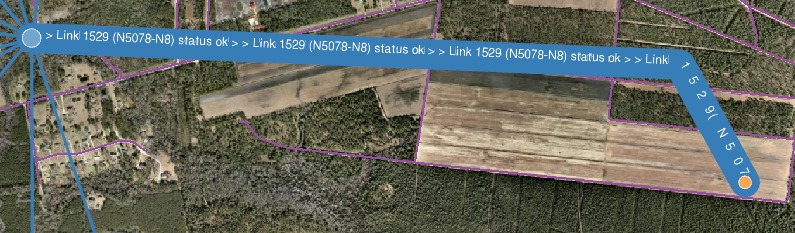
\includegraphics[width=0.8\linewidth]{img/text_path.jpg}
    \caption[Text Drawn on a Path]{An image showing text drawn on an expanded path. The string {\tt ``Link 1529 (N5078-N8) status OK > >''} is repeated over entire length of the path.}
    \label{fig:text_path}
\end{figure}

The individual triangles are then rendered after having the following transformation applied to the positions to line the text up with the path. Each vertex must be translated to the origin by the starting vertex's position, rotated by the calculated amount, and then translated back to original position due to the nature of rotations in OpenGL\@. 

We only need a single VBO for rendering all of the text for the application, even with rotated 
groups of text as described above.

\section{Satellite Images}
\label{section:satellite_images}

The satellite image layer of the visualization handles drawing satellite images at a given level of detail. 
This code required relatively few changes, as the main operations performed when rendering 
these images are independent of OpenGL calls. Andrew Zonenberg previously implemented a tile cache which loads different textures into RAM based on the current level of detail and camera position of the system. At most 10 images are fetched by the CPU and loaded as textures to draw any combination of satellite images for a particular scene. Each of these tiles is drawn as a quadrilateral made up of two triangles. A basic vertex and fragment shader render the textures.

In order to facilitate magnifying the satellite images, we render them to a Frame Buffer 
Object (FBO). FBOs allow for rendering data without immediately drawing this data to the screen. The satellite images are drawn to a texture that is same size as the screen. To render this final texture, we simply draw a quadrilateral that encompasses the entire screen, using the texture created by the FBO\@. 
This final texture does not need a model-view matrix, as we simply define it in terms of projection 
space.

\section{Road Network}
\label{section:road_network}

The previous implementation of rendering the roads in the visualization used an intermediate 
version of {\tt glDrawArrays()} which allowed CPU arrays to be bound as data (Vertex Arrays) to avoid using {\tt glBegin()} and {\tt glEnd()}. The road network was represented as an array of line strips, such that an individual road was either a single line segment for straight roads or multiple line segments for curved roads.

\begin{figure}[htp] \centering
    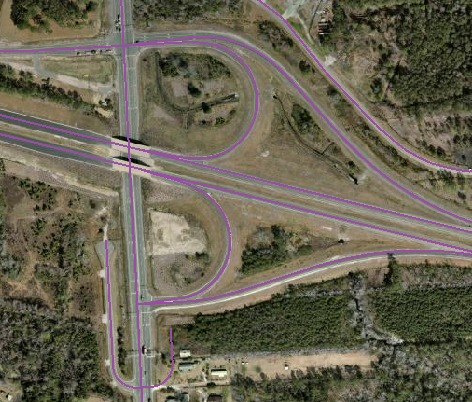
\includegraphics[width=0.8\linewidth]{img/satellite_and_road.jpg}
    \caption[Satellite Images and Roads]{An image showing a curved road, rendered with purple lines, on top of the satellite images.}
    \label{fig:satellite_and_road}
\end{figure}

An initial implementation of changing the rendering of the road network used {\tt glDrawArrays()} with 
these individual line strips. Each individual line strip was bound to a frame buffer and then 
immediately drawn. This rendering method had a negative impact on the overall performance of 
the application, as every invocation of {\tt glBufferData()} requires new data to be allocated. 

To solve the performance issues, the road network was transitioned to the method of rendering 
lines described earlier. All of the line strips are split into individual 
line segments  and stored in a single VBO\@. This new method of rendering allows for a single call to 
{\tt glDrawArrays().} This data is also static for the entire life of the the visualization, so we can improve 
performance even further by only loading the data into the VBO one time and using {\tt GL\_STATIC\_DRAW} 
to notify OpenGL that the data will not be changed after being initialized. The positioning of the road 
network is dependent on the model view projection matrices, and still requires the matrices 
to be passed in as uniform variables to be rendered correctly.

Similar to the satellite images, we render the road network to the FBO to allow the magnification 
to affect the road network.

\section{Summary}
\label{section:methods_summary}

This chapter discussed the changes to the code that were required for our magnification functions to be applied. A brief overview of the changes between legacy OpenGL and modern OpenGL were discussed, followed by the specific changes to the rendering system. The following chapter describes the non-linear magnification function used by our application and its implementation within our systems.
